\documentclass{standalone}
\usepackage{tikz}
\usepackage{ctex,siunitx}
\usepackage{tkz-euclide}
\usepackage{amsmath}
\usetikzlibrary{patterns, calc}
\usetikzlibrary {decorations.pathmorphing, decorations.pathreplacing, decorations.shapes,}
\begin{document}
\small
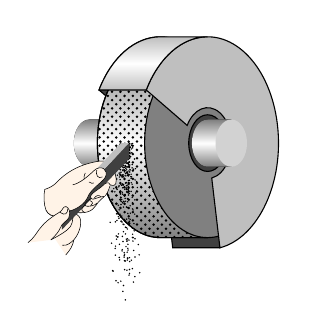
\begin{tikzpicture}[>=latex,scale=1.0]
  % \useasboundingbox (-0.1,0.1) rectangle(6.1,-3.1);
  \fill[top color=gray,bottom color=gray,middle color=white](-1.2,0.3)arc(90:270: 0.2 and 0.3)--(-0.9,-0.3)--(-0.9,0.3);
  \begin{scope}[xshift=-3mm]
    \draw[fill=darkgray]({0.3*cos(150)},{0.45*sin(150)})arc(150:-80:0.3 and 0.45)--({0.9*cos(-80)},{1.35*sin(-80)})--++(0.6,0)--(0.9,0)arc(0:150:0.9 and 1.35)--cycle;
    \end{scope}
  \draw[top color=gray,bottom color=gray,middle color=white](-0.3,1.2)arc(90:270: 0.8 and 1.2)--(0.3,-1.2)--(0.3,1.2)--cycle;
  \draw[pattern= crosshatch dots](-0.3,1.2)arc(90:270: 0.8 and 1.2)--(0.3,-1.2)--(0.3,1.2)--cycle;
  \draw[fill=gray](0.3,0)ellipse(0.8 and 1.2);
  \draw[fill=darkgray](0.3,0)ellipse(0.24 and 0.36);
  \begin{scope}[xshift=3mm]
  \draw[fill=lightgray]({0.3*cos(150)},{0.45*sin(150)})arc(150:-80:0.3 and 0.45)--({0.9*cos(-80)},{1.35*sin(-80)})arc(-80:150:0.9 and 1.35)--cycle;
  \draw[top color=lightgray, bottom color= lightgray,middle color=white]({0.9*cos(150)},{1.35*sin(150)})--++(-0.6,0)arc(150:90:0.9 and 1.35)--++(0.6,0)arc(90:150:0.9 and 1.35)--cycle;
  \end{scope}
  \fill[top color=gray,bottom color=gray,middle color=white](0.3,0.3)arc(90:270: 0.2 and 0.3)--(0.6,-0.3)--(0.6,0.3);
  \fill[lightgray!70](0.6,0)ellipse(0.2 and 0.3);
  
  \foreach \x in {-0.7,-0.75,-0.8}
  {\foreach \y in {1,2,...,70}
  {
    \fill({abs(rand)*0.002*\y+\x},{-abs(rand)*0.03*\y})circle(0.3pt);
    \fill({-abs(rand)*0.002*\y+\x},{-abs(rand)*0.03*\y})circle(0.3pt);
  }
  }
  \draw[fill=pink!10!orange!10,very thin](-1.068,-0.228)..controls(-0.932,-0.208)and(-0.853,-0.379)..
  (-0.863,-0.486)..controls(-0.860,-0.536)and(-0.894,-0.549)..
  (-0.939,-0.529)..controls(-0.983,-0.713)and(-1.033,-0.658)..
  (-1.124,-0.799)..controls(-1.162,-0.857)and(-1.259,-0.922)..
  (-1.447,-0.860)..controls(-1.527,-0.945)and(-1.701,-0.965)..
  (-1.753,-0.850)..controls(-1.781,-0.780)and(-1.785,-0.671)..
  (-1.769,-0.589)..controls(-1.707,-0.566)and(-1.666,-0.546)..
  (-1.624,-0.506)..controls(-1.474,-0.344)and(-1.285,-0.259)..cycle
  (-1.742,-1.058)..controls(-1.621,-0.915)and(-1.421,-0.816)..
(-1.332,-0.933)..controls(-1.293,-0.978)and(-1.308,-1.121)..
(-1.399,-1.229)..controls(-1.414,-1.313)and(-1.448,-1.357)..(-1.502,-1.421);
  \fill[darkgray](-1.55,-0.9)--(-0.7,0)--(-0.7,-0.2)--(-1.55,-1.1);
  \fill[lightgray](-1.55,-0.9)--(-0.7,0)--(-0.8,-0)--(-1.65,-0.9);
  \draw[fill=pink!10!orange!10,very thin](-1.413,-0.530)..controls(-1.314,-0.507)and(-1.218,-0.419)..
  (-1.143,-0.349)..controls(-1.058,-0.266)and(-0.944,-0.340)..
  (-1.003,-0.439)..controls(-1.042,-0.503)and(-1.190,-0.584)..
  (-1.228,-0.698)..controls(-1.255,-0.757)and(-1.345,-0.834)..(-1.447,-0.860)..controls(-1.527,-0.945)and(-1.701,-0.965)..
  (-1.753,-0.850)(-0.939,-0.529)..controls(-0.934,-0.506)and(-0.968,-0.489)..
  (-1.010,-0.519)..controls(-1.077,-0.590)and(-1.168,-0.623)..
  (-1.188,-0.675)..controls(-1.194,-0.692)and(-1.178,-0.720)..
  (-1.137,-0.709)..controls(-1.107,-0.697)and(-1.060,-0.680)..(-1.011,-0.677);
  \draw[very thin](-1.140,-0.701)..controls(-1.130,-0.674)and(-1.081,-0.649)..(-1.058,-0.679)
  (-1.207,-0.494)..controls(-1.175,-0.516)and(-1.157,-0.512)..(-1.146,-0.506)
  (-1.108,-0.342)..controls(-1.126,-0.407)and(-1.090,-0.458)..(-1.037,-0.430)
  (-1.254,-0.379)..controls(-1.273,-0.425)and(-1.273,-0.439)..(-1.267,-0.456)
  (-1.177,-0.705)..controls(-1.210,-0.717)and(-1.260,-0.756)..
(-1.260,-0.783)..controls(-1.260,-0.800)and(-1.240,-0.810)..
(-1.167,-0.796)..controls(-1.138,-0.787)and(-1.115,-0.775)..(-1.105,-0.762)
(-1.191,-0.731)..controls(-1.151,-0.750)and(-1.157,-0.777)..(-1.183,-0.791)
(-1.258,-0.791)..controls(-1.319,-0.836)and(-1.301,-0.860)..(-1.268,-0.877)
(-1.692,-1.229)..controls(-1.564,-1.163)and(-1.476,-1.108)..
(-1.440,-1.056)..controls(-1.420,-1.027)and(-1.419,-0.997)..(-1.411,-0.947)
(-1.545,-1.297)..controls(-1.485,-1.311)and(-1.434,-1.260)..(-1.399,-1.229);
\draw[fill=pink!10!orange!10,very thin]
(-1.982,-1.264)..controls(-1.837,-1.152)and(-1.879,-1.055)..
(-1.577,-0.875)..controls(-1.539,-0.855)and(-1.534,-0.792)..
(-1.495,-0.808)..controls(-1.464,-0.822)and(-1.431,-0.874)..
(-1.465,-0.952)..controls(-1.479,-0.985)and(-1.554,-1.015)..
(-1.570,-1.076)..controls(-1.594,-1.127)and(-1.625,-1.168)..(-1.692,-1.229);
\draw[very thin](-1.574,-0.880)..controls(-1.516,-0.924)and(-1.477,-0.901)..(-1.476,-0.833);
\end{tikzpicture}
\end{document}